\documentclass[a4paper,10pt]{article}
%\documentclass[a4paper,10pt]{scrartcl}

\usepackage[utf8]{inputenc}
\usepackage[brazil]{babel}
\usepackage[T1]{fontenc}
\usepackage[pdftex]{hyperref}
\usepackage{graphicx}
\usepackage{amsmath}
\usepackage{indentfirst}
\usepackage{fancyhdr}
\usepackage{subfig}
\usepackage{setspace}
\usepackage{geometry}
\newcommand{\HRule}{\rule{\linewidth}{0.5mm}}
\usepackage{xcolor}
\usepackage{cite}  % Needed to use citations.  
\definecolor{verde}{rgb}{0.25,0.5,0.35}
\definecolor{jpurple}{rgb}{0.5,0,0.35}
\usepackage{listings}

\lstset{
  language=Java,
  basicstyle=\ttfamily\small,
  keywordstyle=\color{jpurple}\bfseries,
  stringstyle=\color{red},
  commentstyle=\color{verde},
  morecomment=[s][\color{blue}]{/**}{*/},
  extendedchars=true,
  showspaces=false,
  showstringspaces=false,
  numbers=left,
  numberstyle=\tiny,
  breaklines=true,
  backgroundcolor=\color{cyan!10},
  breakautoindent=true,
  captionpos=b,
  xleftmargin=0pt,
  tabsize=4
}
\pagestyle{empty}
% Formatação
\topmargin -1.5cm
\oddsidemargin -0.04cm
\evensidemargin -0.04cm
\textwidth 16.59cm
\textheight 21.94cm 


\pdfinfo{%
  /Title    ()
  /Author   ()
  /Creator  ()
  /Producer ()
  /Subject  ()
  /Keywords ()
}

\begin{document}

\begin{titlepage}

\begin{center}

\includegraphics[width=0.15\textwidth]{./imgs/IME.png}\\[1cm]
\textsc{\Large Instituto de Matemática e Estatística\\ Universidade de São Paulo}\\[0.5cm]
{\large Bacharelado em Ciências da Computação}\\[5.0cm]
\HRule \\[0.4cm]
{\huge \bfseries Library Mapper} 
\HRule \\[1.0cm]

\begin{flushleft} \large
{\large Thiago Gomes Toledo\\ Supervisor: Prof. Dr. Marcelo Finger}
\end{flushleft}
\vfill

{\large São Paulo - SP\\[0.5cm] Segundo semestre de 2011}
\end{center}
\end{titlepage}

\newpage

\textit{ Agradeço a minha mãe Mara Lucia Gomes Toledo e a meu pai João Batista Toledo por terem me dado a oportunidade de realizar 
meu sonho; A minha esposa Lucianna Thomaz Almeida Toledo por me dar conforto, ajuda e sábias dicas; A meu filho que me traz
alegria só por imaginar seu rosto e a Deus por ter me dado todos e tudo que sempre precisei.}


\footnote[1]{Para mais informações sobre essa monografia, apresentação, código, etc.. acesse o site: \href{''http://www.linux.ime.usp.br/~renoir/mac499/proposta.html''}{www.linux.ime.usp.br/~renoir/mac499/proposta.html}}
\newpage
 \tableofcontents
\newpage
    \section{Introdução}
   
    Como frequentador da biblioteca do Instituto de Matemática e 
    Estatística da USP desde 2008 e trabalhando na biblioteca do Instituto de Geociencias da USP em 2010-2012, 
    pude notar que as reclamações numa biblioteca sobre a dificuldade em se achar um livro lideram o ranking de 
    problemas apontados por visitantes que usualmente têm que apelar para a boa vontade dos funcionários, 
    pois acham muito complicado ou até sem nenhum sentido o modo como as fileiras de livros são identificadas.
    
    Em ambos os casos os alunos ainda eram capazes de encontrar seus livros ou teses dado que a maior delas possuia
    não mais que 20.000 exemplares.Contudo, numa biblioteca como a da Faculdade de Filosofia, Letras e Ciências Humanas
    que hoje possui um inventório de mais de 500 mil livros e ainda 600 mil teses\footnote[1]{Dados levantados em janeiro 2012 com a diretora da biblioteca, Maria Aparecida Laet}, a busca se torna completamente inviável
    sem nenhum auxílio real.
   
    
    \section{Parte Objetiva}
    Nessa parte do texto, serão apresentados os conceitos teóricos do trabalho, além da parte prática
    de desenvolvimento.

    \subsection{Objetivo}
    Com uma ferramenta que mostre como ir do ponto onde está o visitante até o livro através de um mapa, esse dificilmente se sentiria perdido 
    ou precisaria contar com o auxílio de terceiros.Portanto, o objetivo desse projeto Library Mapper é que o vistante
    busque, escolha o livro e receba no seu aparelho mobile um mapa com o caminho correto até esse livro.
    
    \subsection{Problema}

    Como dispositivos GPS não mapeam dentro de residências, é inviável utilizar a Geolocalização do visitante para qualquer fim e portanto
    era necessário criar algum método para identificar onde ele estava localizado, como era esse lugar e como gerar uma busca
    entre onde ele estava e onde devia chegar.
    
    
    \subsection{Solução}
    
  Inicialmente desenvolvida para dispositivos IOS, essa ferramenta utiliza tags com códigos QR para auxiliar 
  o reconhecimento da localização atual do visitante.
  O visitante ao entrar numa biblioteca procura essa tag e com seu dispositivo IOS, reconhece o código 
  nela contido.Esse código abre um Web Browser no dispositivo e uma página da biblioteca na internet é 
  mostrada na tela.O visitante digita o livro num campo de busca e uma vez que esse existe nessa biblioteca, 
  a tela do web browser é substituída por uma tela com um mapa que mostra o caminho da tag selecionada 
  até a fileira onde esta o livro.
  
   Para ser possível a localização do livro, será utilizada a prévia catalogação feita pela biblioteca da 
   posição do mesmo e uma réplica proporcional do mapa real da biblioteca .Essa réplica
   é desenvolvida através de uma plataforma web que gera mapas 2D também desenvolvida nesse projeto.As informações
   obtidas nesse mapa, localização de estantes e suas correspondentes identificações, Qr-Codes, obstáculos e limites
   da biblioteca, serão enviados e armazenados num banco de dados da aplicação.\\
   
   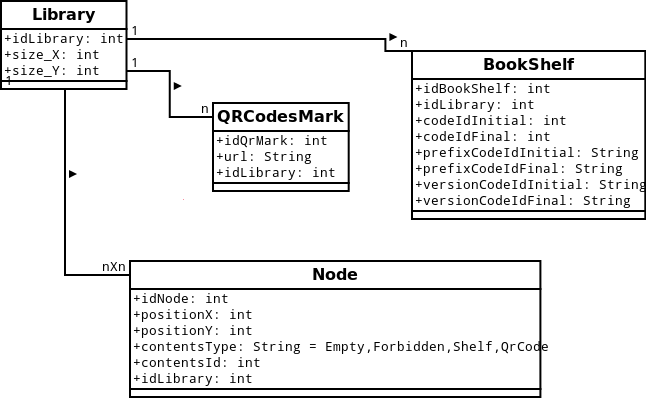
\includegraphics[width=0.70\textwidth]{./imgs/merLibraryMappper.png}\\[1cm]
   
   
   O mapa será gerado num grafo tipo grid e cada nó está dividido em 4 tipos principais que são QR-Code, Forbidden, Free e Bookshelf 
   numa classe Node e será baseado nesses tipos que a busca pelo livro dado será feita.

   Como todas as arestas destre grafo tem peso único um, o algoritmo de busca usado é uma Bi-direcional BFS (Breadth-first search) com uma busca saindo da origem(QR-Code
   selecionado pelo visitante) e outra do destino (estante onde está o livro).\\

Essa busca é feita de uma maneira paralela onde cada thread é um dos pólos do caminho Bi-direcional.\\ 
  
    \subsection{Conceitos e tecnologias estudadas}
      \subsubsection{O que são Qr-Codes?}
      Quick Response Code foi inventado por \href{http://www.denso-wave.com/}{DENSO WAVE}, uma empresa Japonesa de captura automática de dados, FA e campos de solução de negócios, em 1994 e foi um dos primeiros códigos de barra 2D
      a ser usado em aplicações onde era necessário uma combinação de camera de aparelhos celulares e códigos de barra 2D.\cite{barcode}Esses códigos trocam barras e espaços
      por pontos e espaços arranjados num vetor ou uma matrix, aumentando consideravelmente a quantidade de dados
      armazenados num espaço igualmente usado para um código de barra 1D.
      Apenas em 2002 cameras de celulares foram comercialmente vendidas com dispositivos reconhecedores de Qr-codes e desde
      então uma vasta variedade de aplicativos começou a surgir no Japão e vem tomando o mundo.\\[0.80cm]
      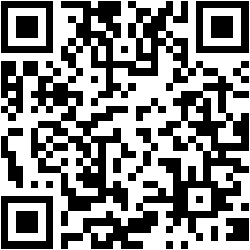
\includegraphics[width=0.30\textwidth]{./imgs/qrcode.png} .Em 2006, como parte do Windows Live service, a Microsoft lançou o Windows Live Barcode
      , onde Qr-codes eram usados como ponte para troca de informações entre aparelhos mobile e outras medias como PCs, Tv de plasma
      e revistas.
      
      As Qr-Codes geradas para esse projeto passarão para o usuário o endereço de uma página web de busca dos livros da 
      bilioteca em que ele se encontra.Junto nessa URL tem um id do Qr-Code, que mostra para o programa onde no grafo
      do mapa da biblioteca se encontra o visitante, para dessa maneira poder criar o caminho que o mesmo deve traçar.
      
      
      
      \subsubsection{Grid Graphs}
      
      Um grafo \textit{G} é uma par \textit{(V,E)}, onde \textit{V} é um conjunto finito e \textit{E} é uma relação binária de \textit{V}.
      O conjunto \textit{V} é chamado de o \textit{conjunto de vértices} de \textit{G} e seus elementos são chamados 
      de \textit{vértices}.O conjunto \textit{E} é chamado de \textit{conjunto de arestas} de \textit{G} e seus elementos
      são chamados de \textit{arestas}.Existem dois tipos de grafos - grafo direcionados e grafos não-direcionados.
            \cite{bfs}
      
      Uma aresta num \textit{grafo não-direcionado} é um conjunto \textit{\{u,v\}} onde \textit{u,v} $\in$ \textit{V} e \textit{u $\neq$ v} que por
      convenção é definida como \textit{$(u,v)$} ou \textit{$(v,u)$} e é possível ir de \textit{u} para \textit{v} e de \textit{v} 
      para \textit{u}.
      
      Já num \textit{grafo direcionado} (ou \textit{dígrafo} ) uma aresta é identificada por setas e \textit{$(u,v)$} \textit{$\neq$} \textit{$(v,u)$}.
     
      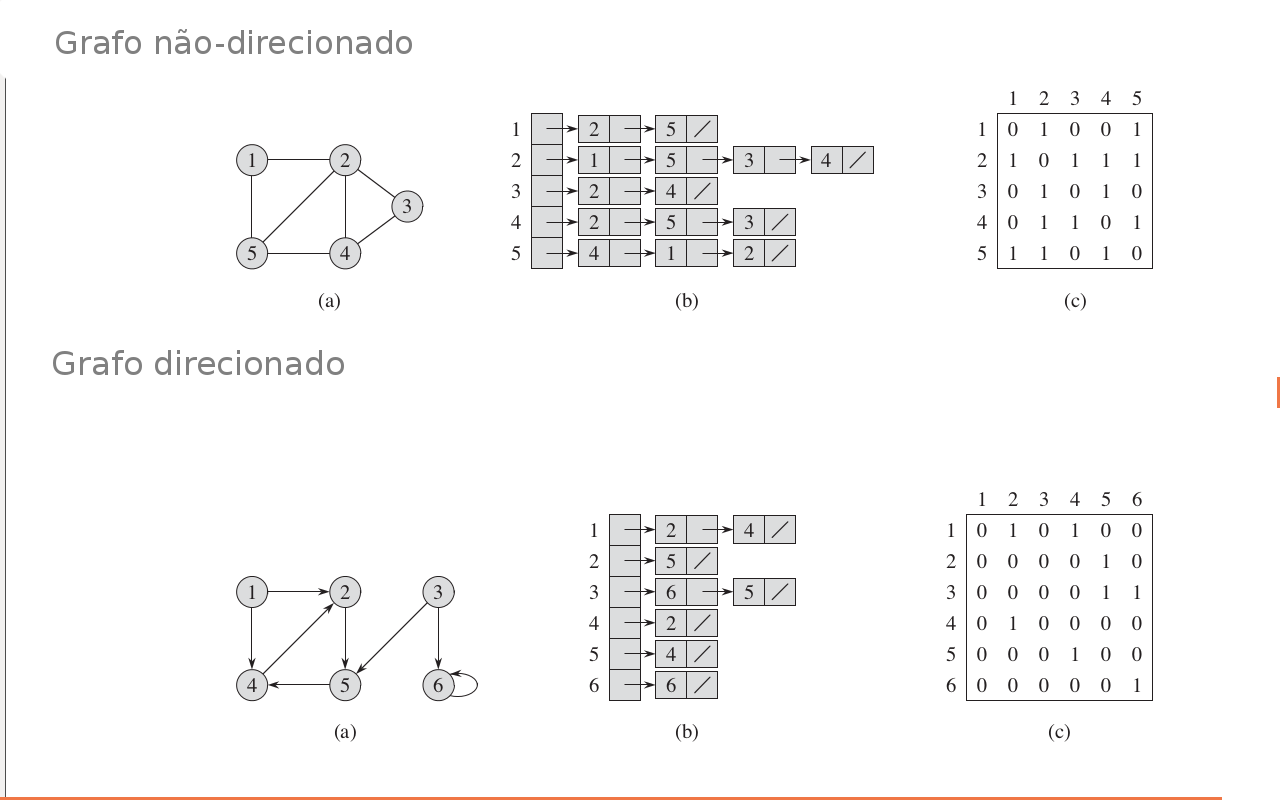
\includegraphics[width=0.9\textwidth]{./imgs/grafo.png}\\[1cm]
      
      Em ambos os casos uma aresta \textit{(u,v)} pode possuir um \textit{peso} que indica o custo por passar do vértice \textit{u}
      para o \textit{v}.
      
      Um Grid Graph ( grafo do tipo Grid ) é um grafo não-direcionado; uma grade de nós (vértices) \textit{n} x \textit{n} sendo que cada
      nó tem exatamente 4 arestas com exceção dos nós das extremidades.
      
      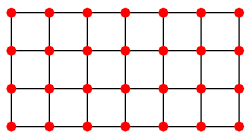
\includegraphics[width=0.5\textwidth]{./imgs/grid.png}\\[1cm]
      Para o LibraryMapper será usado um grafo não-direcinado do tipo Grid alocado numa matriz, sendo que cada vértice do grafo 
      será um nó da classe Node.Essa Possui os seguintes atributos:
      
      
      \begin{lstlisting}
package library.domain;

public class Node {

    private Integer idNode;
    private Integer positionX;
    private Integer positionY;
    private Integer contentId;
    private Integer idLibrary;
    private String contentType;
    private Node parentFromBeginNode;
    private Node parentFromEndNode;
    private int mapValue;
    
/*... continua ...*/
\end{lstlisting}
      
      
      
      
      \subsubsection{Breadth-First Search (BFS)}
      Dado um grafo \textit{G=(V,E)} com um vértice \textit{s} distinto, Breadth-first search explora sistematicamente
      as arestas de \textit{G} para descobrir todo vértice que pode ser alcançado por \textit{s}.Ele computa a distância
      (menor número de arestas) do vértice \textit{s} até todos os vértices que ele possa alcançar.Para manter o controle do progresso da busca, BFS procura cores em cada vértice - branco, cinza e preto. Todos os 
      vértices começam com cor branca, eventualmente passam para cinza e por fim  ficam pretos.\cite{bfs}
      
      Uma vez que um vértice é descoberto ele se torna não-branco.Um vértice só se tornará preto quando todos os vértices
      que são adjacentes á ele tenham sido descobertos, enquanto isso ele será cinza.Isso representa a fronteira entre
      vértices descobertos e não-descobertos.\\
	
	Como no pior caso, a busca tem que ser feita em todos os m nós de um grafo e como a 
      BFS passa não volta nos caminhos que já traçou, a complexidade desse algoritmo é O(m).	 
      \begin{figure}
	\centering
      	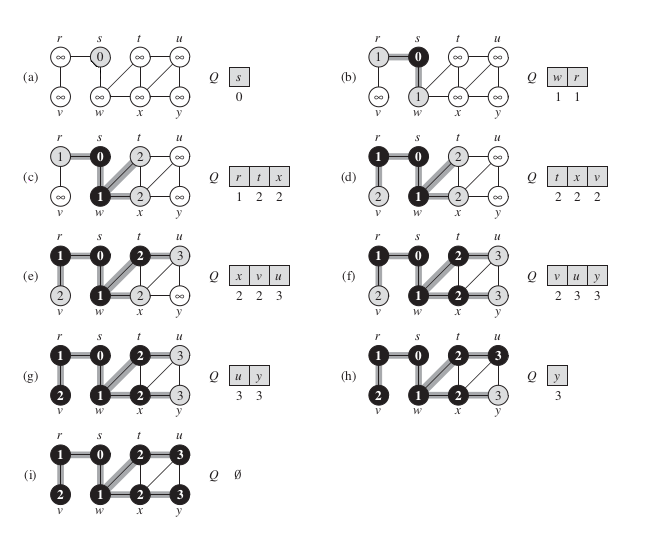
\includegraphics[width=0.70\textwidth]{./imgs/bfs.png}
	\caption{BFS retirada do livro X}
      \end{figure}
      Além das cores, nesse projeto essa BFS distingue entre nós (vértices) do tipo Free, Bookshelf, Qr-Code e Forbidden e será 
      aplicada de uma maneira Bi-direcional.
      
      \subsubsection{Bi-directional BFS}
	A idéia por trás de uma busca Bi-direcional é fazer duas buscas rodarem simultaneamente - Uma "para frente", 	 
	saindo do estado inicial (a origem) da busca inteira e outra "para trás",  saindo do estado final ( a chegada ) 
	da busca inteira esperando que ambas se encotrem no meio.\cite{bidirecional}.\\[0.8cm] 

	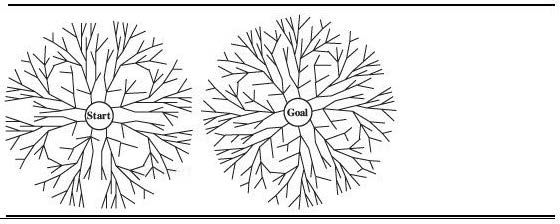
\includegraphics[width=1.0\textwidth]{./imgs/bi-directional.png}\\[1cm]   
	Nesse projeto a busca Bi-direcional será realizada através de métodos concorrentes de programação.Cada pólo
	iniciará sua busca paralelamente liberando assim duas threads.Caso uma thread chegue em um nó que já foi 
	visitado ela define aquele nó como o "meio do caminho" e a partir dele gera a rota inteira do mapa.Mas caso o nó que
	chegue esteja sendo visitado, ela para e abandona o que estiver fazendo para depois ser reciclada num outro novo processo. 
	\\Pela profundidade da busca ter caído pela metade, ou seja, no máximo uma busca tem que ir até a metade do grafo, a complexidade do algoritmo é O(m/2).
	
	\subsubsection{MER - Modelo Entidade Relacionamento}
	\subsubsection{PgAdmin - }
	\subsubsection{POO - Programação Orientada a Objetos}
	\subsubsection{Mybatis - Integração MER e POO}
	\subsubsection{Servlet - WebService JAVA}
	\subsubsection{Apache Tomcat - Servidor WEB}
	\subsubsection{Métodos Ágeis - Kanban e Integração Contínua}
	\subsubsection{HTML5 - Canvas}
      	\subsubsection{Desenvolvimento mobile}
	
   \subsection{Library Mapper, o cliente}
	\subsubsection{Construindo o seu mapa Web}
	\subsubsection{Transformação do JavaScript para Nodes}
	\subsubsection{Salvando no Banco de Dados}
   \subsection{Library Mapper, o usuário}
	\subsubsection{Identificando o usuário}
	\subsubsection{A consulta e a ligação com a biblioteca}
	\subsubsection{Lista de livros e a busca pela estante}
	\subsubsection{Montando o mapa com HTML5 e canvas}
   \subsection{Atividades realizadas}
	
   \subsection{Resultados e produtos obtidos}
   \subsection{Conclusões}

   
  \section{Parte Subjetiva}
  \subsection{Desafios e frustrações}
  \subsection{Relações entre Disciplinas}
  \subsection{Os próximos passos}
  
  
\bibliographystyle{plain}   
\bibliography{refer}
\end{document}
